% Options for packages loaded elsewhere
\PassOptionsToPackage{unicode}{hyperref}
\PassOptionsToPackage{hyphens}{url}
%
\documentclass[
]{article}
\usepackage{amsmath,amssymb}
\usepackage{iftex}
\ifPDFTeX
  \usepackage[T1]{fontenc}
  \usepackage[utf8]{inputenc}
  \usepackage{textcomp} % provide euro and other symbols
\else % if luatex or xetex
  \usepackage{unicode-math} % this also loads fontspec
  \defaultfontfeatures{Scale=MatchLowercase}
  \defaultfontfeatures[\rmfamily]{Ligatures=TeX,Scale=1}
\fi
\usepackage{lmodern}
\ifPDFTeX\else
  % xetex/luatex font selection
\fi
% Use upquote if available, for straight quotes in verbatim environments
\IfFileExists{upquote.sty}{\usepackage{upquote}}{}
\IfFileExists{microtype.sty}{% use microtype if available
  \usepackage[]{microtype}
  \UseMicrotypeSet[protrusion]{basicmath} % disable protrusion for tt fonts
}{}
\makeatletter
\@ifundefined{KOMAClassName}{% if non-KOMA class
  \IfFileExists{parskip.sty}{%
    \usepackage{parskip}
  }{% else
    \setlength{\parindent}{0pt}
    \setlength{\parskip}{6pt plus 2pt minus 1pt}}
}{% if KOMA class
  \KOMAoptions{parskip=half}}
\makeatother
\usepackage{xcolor}
\usepackage[margin=1in]{geometry}
\usepackage{graphicx}
\makeatletter
\def\maxwidth{\ifdim\Gin@nat@width>\linewidth\linewidth\else\Gin@nat@width\fi}
\def\maxheight{\ifdim\Gin@nat@height>\textheight\textheight\else\Gin@nat@height\fi}
\makeatother
% Scale images if necessary, so that they will not overflow the page
% margins by default, and it is still possible to overwrite the defaults
% using explicit options in \includegraphics[width, height, ...]{}
\setkeys{Gin}{width=\maxwidth,height=\maxheight,keepaspectratio}
% Set default figure placement to htbp
\makeatletter
\def\fps@figure{htbp}
\makeatother
\setlength{\emergencystretch}{3em} % prevent overfull lines
\providecommand{\tightlist}{%
  \setlength{\itemsep}{0pt}\setlength{\parskip}{0pt}}
\setcounter{secnumdepth}{-\maxdimen} % remove section numbering
\usepackage{booktabs}
\usepackage{longtable}
\usepackage{array}
\usepackage{multirow}
\usepackage{wrapfig}
\usepackage{float}
\usepackage{colortbl}
\usepackage{pdflscape}
\usepackage{tabu}
\usepackage{threeparttable}
\usepackage{threeparttablex}
\usepackage[normalem]{ulem}
\usepackage{makecell}
\usepackage{xcolor}
\usepackage{placeins}
\usepackage{booktabs}
\usepackage{longtable}
\usepackage{array}
\usepackage{multirow}
\usepackage{wrapfig}
\usepackage{float}
\usepackage{colortbl}
\usepackage{pdflscape}
\usepackage{tabu}
\usepackage{threeparttable}
\usepackage{threeparttablex}
\usepackage[normalem]{ulem}
\usepackage{makecell}
\usepackage{xcolor}
\ifLuaTeX
  \usepackage{selnolig}  % disable illegal ligatures
\fi
\IfFileExists{bookmark.sty}{\usepackage{bookmark}}{\usepackage{hyperref}}
\IfFileExists{xurl.sty}{\usepackage{xurl}}{} % add URL line breaks if available
\urlstyle{same}
\hypersetup{
  pdftitle={event-study},
  pdfauthor={Shadi},
  hidelinks,
  pdfcreator={LaTeX via pandoc}}

\title{event-study}
\author{Shadi}
\date{2023-06-27}

\begin{document}
\maketitle

\hypertarget{result-for-event-study-and-parallel-trend}{%
\subsection{Result for event Study and Parallel
trend}\label{result-for-event-study-and-parallel-trend}}

The main assumption of the Difference-in-Differences (DiD) methodology
relies on the presence of parallel trends before the policy
implementation.We examine the event-study estimates for uninsured rates
and Medicaid take-up to assess the impact of Medicaid expansion on
low-income individuals aged 26-64 and assess the validity of parallel
trend assumption.

\hypertarget{event-studies-for-uninsured-rate.-low-income-aged-26-64}{%
\subsubsection{Event studies for Uninsured rate. Low-income aged
26-64}\label{event-studies-for-uninsured-rate.-low-income-aged-26-64}}

Figure 1 displays the event-study estimates for both unconditional and
conditional parallel trends in uninsured rates. In Panel (a), the focus
is on the effects of the expansion on uninsured rates for US-born
individuals, while Panel (b) examines the effects for foreign-born
individuals. The green line with circles in both panels represents the
conditional models, while the orange line with triangle represents the
unconditional models. For the corresponding estimation coefficients,
please refer to Table 1.

As shown in Figure 1, there are no significant pre-trend differences for
US-born individuals living in expansion states compared to non-expansion
states, as the coefficients are not significantly different from zero.
Similarly, for foreign-born individuals, the coefficients for the
interaction terms between year and the indicator for the pre-treatment
period are also small and not statistically significant, indicating no
significant pre-trend differences in the uninsured rates between
foreign-born individuals in expansion states and non-expansion states.
Moreover, when controlling for characteristics, the coefficients exhibit
minimal changes and remain small, further supporting the parallel trend
assumption. Additionally, these coefficients do not attain statistical
significance, indicating that the characteristics accounted for do not
significantly impact the parallel trends assumption.

Transitioning to the post-expansion years, we observe notable and
statistically significant declines in the overall uninsured rates for
both foreign-born and US-born individuals. The coefficients associated
with the indicator variables representing the post-expansion years are
negative and demonstrate statistical significance for both groups. These
results indicate a clear reduction in uninsured rates following the
implementation of Medicaid expansion.

Upon analyzing the results presented in Table 1, it becomes evident that
the significance levels of the lag year coefficients tend to be higher
for foreign-born individuals compared to US-born individuals.
Specifically, in Model 3, the coefficient for the lag year achieves
statistical significance at the 5 level for the foreign-born group. In
Model 4, it reaches statistical significance at the 0.1 level. In
contrast, for the US-born group, the coefficient remains statistically
insignificant in both models. These findings suggest stronger evidence
of a pre-trend difference in uninsured rates for foreign-born
individuals in expansion states compared to non-expansion states, even
after accounting for foreign-born specific characteristics. Conversely,
the evidence for a pre-trend difference in uninsured rates among US-born
individuals is comparatively weaker. The differences in significance
levels indicate a potential violation of the parallel trend assumption
to a greater extent for foreign-born individuals, implying possible
disparities in uninsured rates between expansion and non-expansion
states even prior to the implementation of Medicaid expansion.

The event study presented in Figure 1 indicates significant improvements
in insurance coverage within the expansion states compared to the
non-expansion states following the implementation of Medicaid expansion.
However, the observed divergence in uninsured trends and the relatively
smaller reduction in the uninsured rate for foreign-born individuals
highlight potential disparities in healthcare access. Nevertheless, it
is important to note that the gap between the insured rates of
foreign-born and US-born individuals started to close after 2018.

\begin{verbatim}
## The variables 'CITNaturalized-citizen', 'CITNon-citizen' and 'CITUS-citizen Born abroad ' have been removed because of collinearity (see $collin.var).
\end{verbatim}

\begin{verbatim}
## The variables 'CITBorn in US Territories', 'CITUS-citizen Born abroad ' and 'CORIGINUnited States' have been removed because of collinearity (see $collin.var).
\end{verbatim}

\begin{center}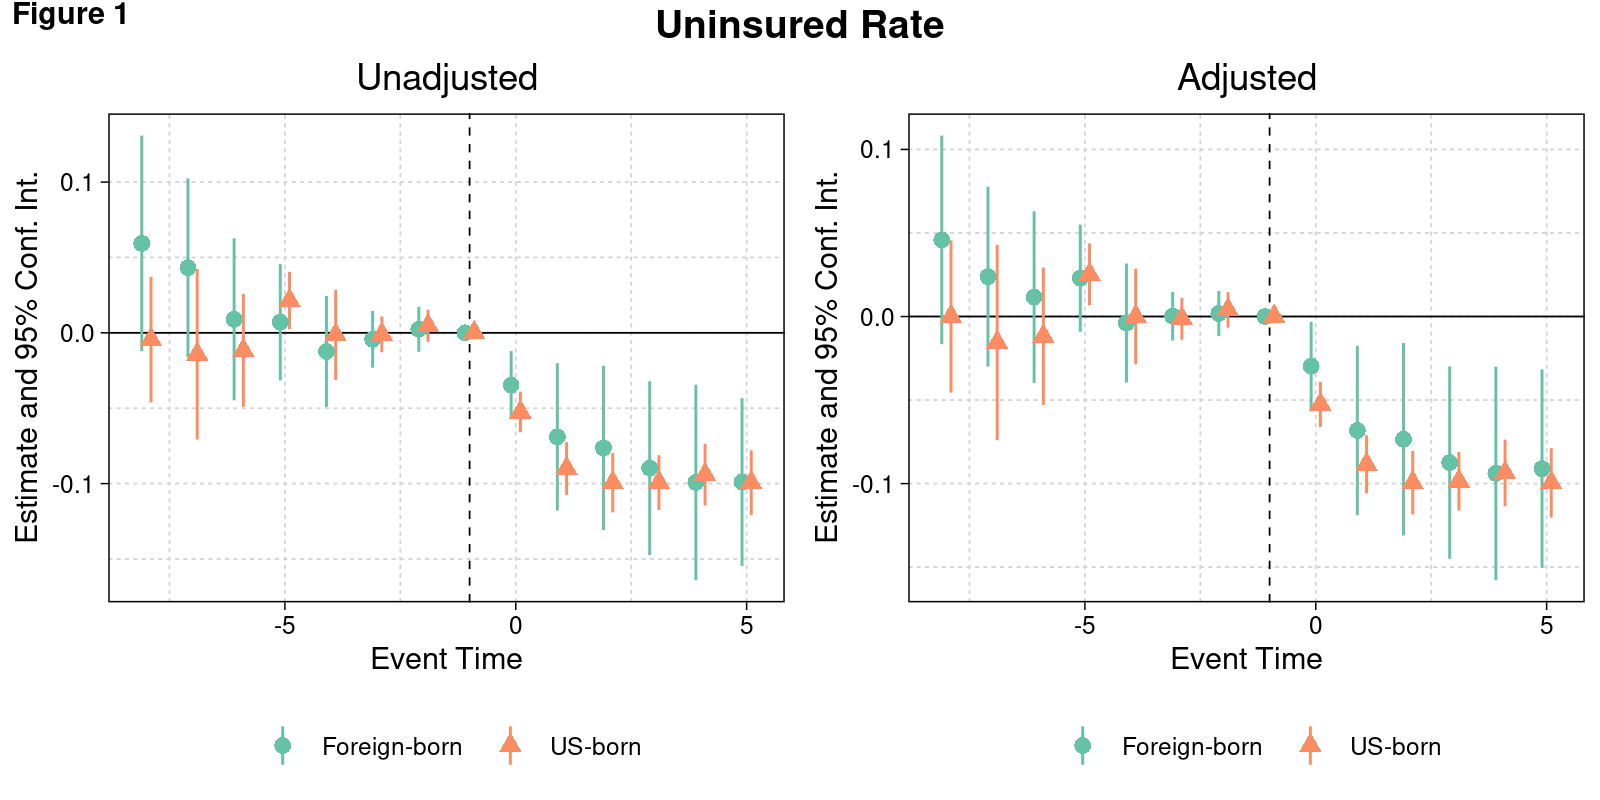
\includegraphics{/home/shadi/Projects/GitHub/medicaid-foreign-born/output/fig1-1} \end{center}

\begin{center}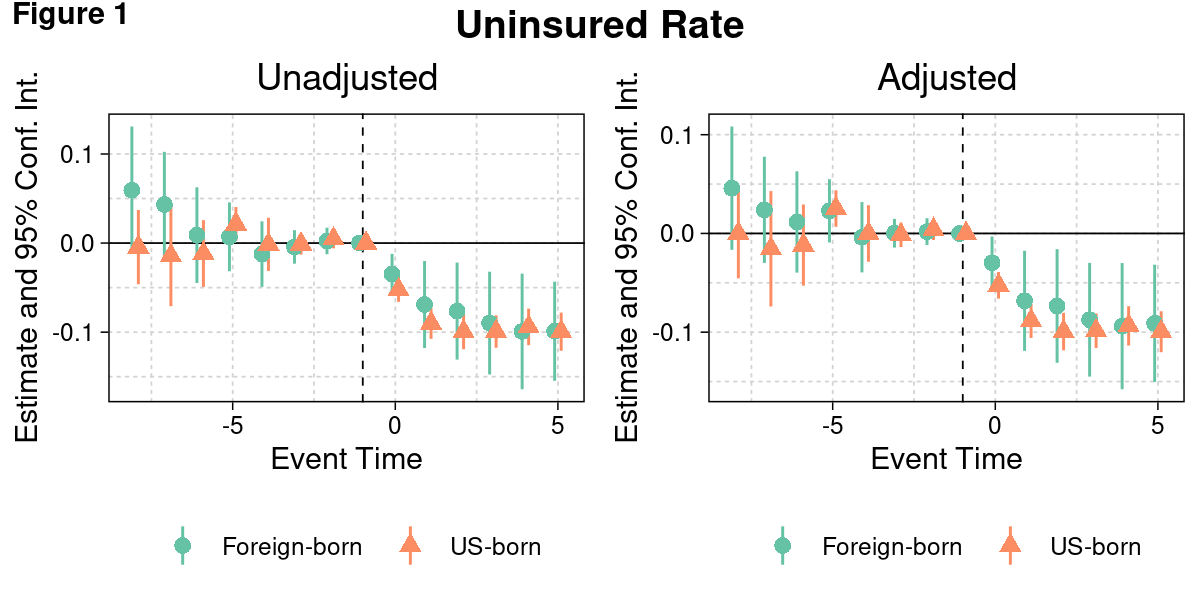
\includegraphics{/home/shadi/Projects/GitHub/medicaid-foreign-born/output/fig1-2} \end{center}
\FloatBarrier

\begin{verbatim}
## Variance contained negative values in the diagonal and was 'fixed' (a la Cameron, Gelbach & Miller 2011).
## Variance contained negative values in the diagonal and was 'fixed' (a la Cameron, Gelbach & Miller 2011).
## Variance contained negative values in the diagonal and was 'fixed' (a la Cameron, Gelbach & Miller 2011).
## Variance contained negative values in the diagonal and was 'fixed' (a la Cameron, Gelbach & Miller 2011).
\end{verbatim}

\begin{table}[htbp]
   \caption{The Impact of Medicaid Expansion on Uninsured Rate }
   \centering
   \small
   \begin{tabular}{lcccc}
      \tabularnewline \midrule \midrule
       & \multicolumn{2}{c}{US-born} & \multicolumn{2}{c}{Foreign-Born} \\ \cmidrule(lr){2-3} \cmidrule(lr){4-5}
      Variables             & (1)            & (2)                    & (3)            & (4)\\  
      \midrule 
      expansion year $=$ -8 & -0.005         & $3.95\times 10^{-5}$   & 0.059$^{*}$    & 0.046\\   
                            & (0.021)        & (0.023)                & (0.030)        & (0.028)\\   
      expansion year $=$ -7 & -0.014         & -0.015                 & 0.043          & 0.024\\   
                            & (0.025)        & (0.026)                & (0.028)        & (0.025)\\   
      expansion year $=$ -6 & -0.012         & -0.012                 & 0.009          & 0.012\\   
                            & (0.019)        & (0.021)                & (0.026)        & (0.026)\\   
      expansion year $=$ -5 & 0.021$^{*}$    & 0.025$^{**}$           & 0.007          & 0.023\\   
                            & (0.011)        & (0.011)                & (0.018)        & (0.016)\\   
      expansion year $=$ -4 & -0.001         & $-2.61\times 10^{-5}$  & -0.012         & -0.004\\   
                            & (0.017)        & (0.017)                & (0.016)        & (0.017)\\   
      expansion year $=$ -3 & -0.001         & -0.001                 & -0.004         & 0.0002\\   
                            & (0.004)        & (0.005)                & (0.010)        & (0.009)\\   
      expansion year $=$ -2 & 0.005          & 0.004                  & 0.002          & 0.002\\   
                            & (0.003)        & (0.004)                & (0.008)        & (0.007)\\   
      expansion year $=$ 0  & -0.052$^{***}$ & -0.053$^{***}$         & -0.035$^{***}$ & -0.030$^{**}$\\   
                            & (0.005)        & (0.005)                & (0.008)        & (0.011)\\   
      expansion year $=$ 1  & -0.090$^{***}$ & -0.088$^{***}$         & -0.069$^{**}$  & -0.068$^{**}$\\   
                            & (0.008)        & (0.008)                & (0.024)        & (0.024)\\   
      expansion year $=$ 2  & -0.100$^{***}$ & -0.100$^{***}$         & -0.076$^{**}$  & -0.073$^{**}$\\   
                            & (0.009)        & (0.009)                & (0.026)        & (0.027)\\   
      expansion year $=$ 3  & -0.099$^{***}$ & -0.099$^{***}$         & -0.090$^{**}$  & -0.087$^{**}$\\   
                            & (0.008)        & (0.008)                & (0.028)        & (0.028)\\   
      expansion year $=$ 4  & -0.094$^{***}$ & -0.094$^{***}$         & -0.099$^{**}$  & -0.094$^{**}$\\   
                            & (0.009)        & (0.009)                & (0.030)        & (0.030)\\   
      expansion year $=$ 5  & -0.100$^{***}$ & -0.100$^{***}$         & -0.099$^{***}$ & -0.091$^{**}$\\   
                            & (0.009)        & (0.009)                & (0.026)        & (0.027)\\   
       \\
      State FE              & yes            & yes                    & yes            & yes\\  
      Year FE               & yes            & yes                    & yes            & yes\\  
      Controls              &                & yes                    &                & yes\\  
      Observations          & 1,585,639      & 1,585,639              & 389,955        & 389,955\\  
      R$^2$                 & 0.05930        & 0.11985                & 0.08577        & 0.21524\\  
      Within R$^2$          & 0.00286        & 0.06704                & 0.00172        & 0.14309\\  
      \midrule \midrule
      \multicolumn{5}{l}{\emph{Clustered (State \& Year) standard-errors in parentheses}}\\
      \multicolumn{5}{l}{\emph{Signif. Codes: ***: 0.01, **: 0.05, *: 0.1}}\\
   \end{tabular}
\end{table}

\hypertarget{event-study-for-medicaid-take-up}{%
\subsubsection{Event Study for medicaid-take
up}\label{event-study-for-medicaid-take-up}}

Figure 2 and Table 2 present the event-study estimates for the
unconditional and conditional parallel trends concerning Medicaid
take-up. According to the data presented in Figure 2,prior to the
implementation of Medicaid expansion, there is no significant pre-trend
difference in Medicaid take-up between expansion and non-expansion
states for both low-income US-born and foreign-born individuals aged
26-64.

For the US-born sub-sample, Model 2 includes control variables, while
Model 1 serves as a baseline model. The coefficients for the interaction
terms between year and the indicator for the pre-treatment period were
generally small and statistically insignificant in both models. This
suggests that there is no significant pre-trend difference in uninsured
rates between expansion and non-expansion states for US-born
individuals.

Similarly, for the foreign-born sub-sample, Model 4 includes control
variables, while Model 3 serves as a baseline model. The coefficients
for the interaction terms were also small and statistically
insignificant in both models, suggesting no significant pre-trend
difference in uninsured rates between expansion and non-expansion states
for foreign-born individuals.

Furthermore, the coefficients for the interaction terms representing the
post-treatment periods (years 0 to 5 after the implementation of
Medicaid expansion) were positive and statistically significant in all
models, indicating an increase in uninsured rates for both US-born and
foreign-born individuals in expansion states compared to non-expansion
states during those years.

Analyzing the results presented in Table 2, a notable pattern emerges
regarding the Medicaid take-up rates between foreign-born and US-born
individuals following the expansion. Initially, during the first three
years after the expansion, the Medicaid take-up rate for foreign-born
individuals was lower compared to that of US-born individuals. However,
a reversal in this observation occurred from year 4 onwards, as the rate
of take-up among foreign-born individuals increased.This suggests that
over time, foreign-born individuals were able to overcome some of the
barriers and obstacles they initially encountered, leading to a higher
participation in Medicaid. It is likely that various factors contributed
to this trend. Changes in immigration policies, targeted outreach
efforts aimed at foreign-born populations, or the implementation of
programs specifically designed to enhance healthcare access for
immigrants could have played a role in facilitating the increased
participation among foreign-born individuals. Further investigation into
the specific policies and initiatives implemented during this period
would provide a deeper understanding of the factors influencing the
changing Medicaid take-up rates among foreign-born individuals. however,
it is surprising to see a higher Medicaid take-up rate for foreign-born
individuals during the fourth and fifth years after expansion, which
align with the years 2018 and 2019 when stricter immigration policies
were implemented under the Trump administration

These findings demonstrate the effectiveness of Medicaid expansion in
improving access to healthcare, especially among foreign-born
individuals. The absence of significant pre-trend differences and the
subsequent increase in Medicaid take-up rates following the expansion
highlight the positive impact of the expansion in reducing the uninsured
population and promoting healthcare coverage for both US-born and
foreign-born individuals in expansion states compared to non-expansion
states.

\begin{verbatim}
## The variables 'CITNaturalized-citizen', 'CITNon-citizen' and 'CITUS-citizen Born abroad ' have been removed because of collinearity (see $collin.var).
\end{verbatim}

\begin{verbatim}
## The variables 'CITBorn in US Territories', 'CITUS-citizen Born abroad ' and 'CORIGINUnited States' have been removed because of collinearity (see $collin.var).
\end{verbatim}

\begin{center}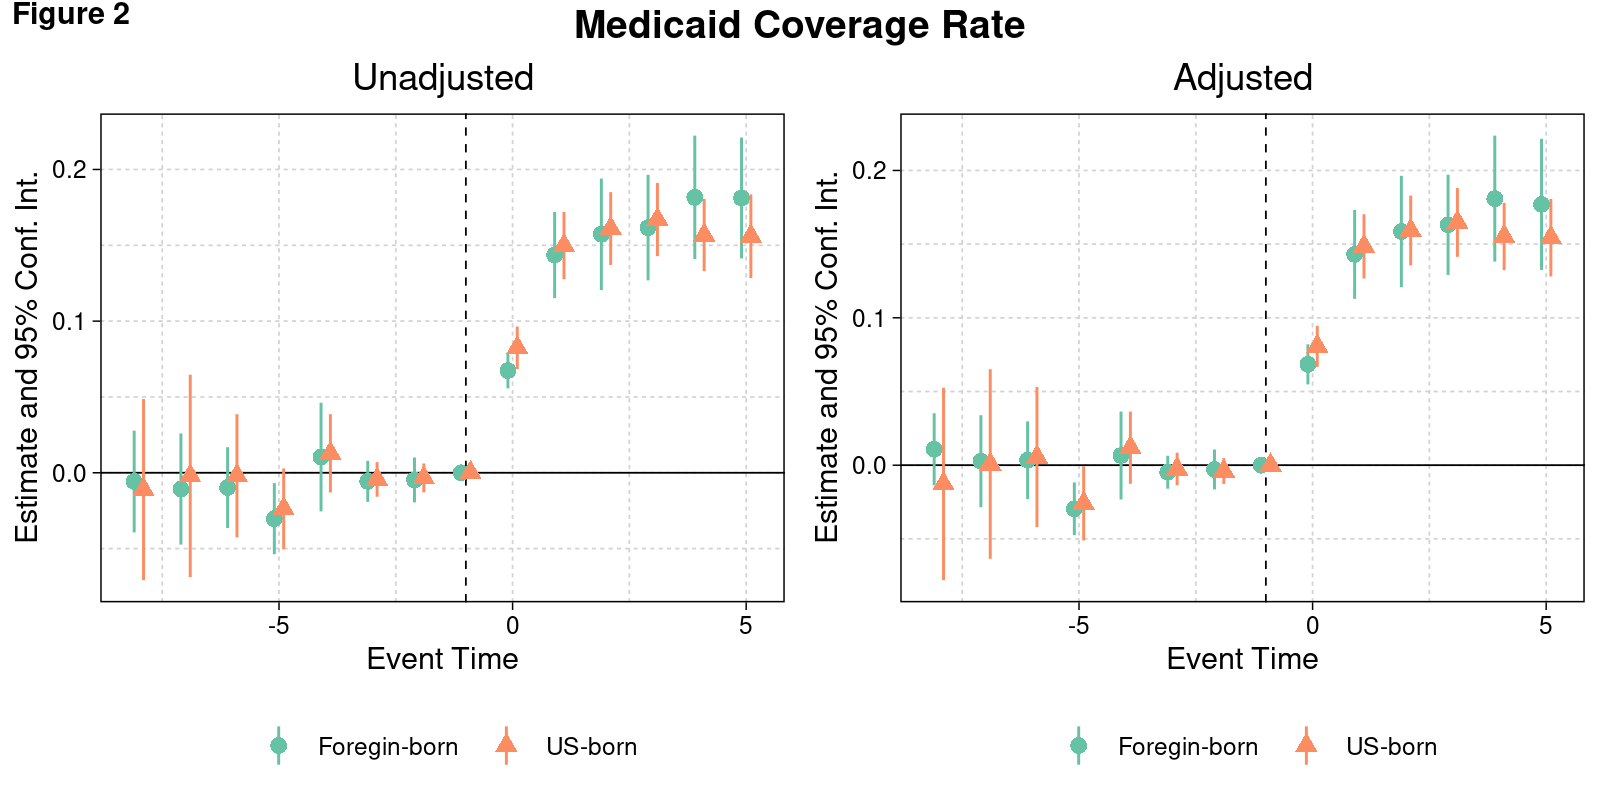
\includegraphics{/home/shadi/Projects/GitHub/medicaid-foreign-born/output/fig2-1} \end{center}

\FloatBarrier

\begin{verbatim}
## Variance contained negative values in the diagonal and was 'fixed' (a la Cameron, Gelbach & Miller 2011).
## Variance contained negative values in the diagonal and was 'fixed' (a la Cameron, Gelbach & Miller 2011).
## Variance contained negative values in the diagonal and was 'fixed' (a la Cameron, Gelbach & Miller 2011).
## Variance contained negative values in the diagonal and was 'fixed' (a la Cameron, Gelbach & Miller 2011).
\end{verbatim}

\begin{table}[htbp]
   \caption{The Impact of Medicaid Expansion on Medicaid Coverage }
   \centering
   \small
   \begin{tabular}{lcccc}
      \tabularnewline \midrule \midrule
       & \multicolumn{2}{c}{US-born} & \multicolumn{2}{c}{Foreign-Born} \\ \cmidrule(lr){2-3} \cmidrule(lr){4-5}
      Variables             & (1)           & (2)           & (3)            & (4)\\  
      \midrule 
      expansion year $=$ -8 & -0.011        & -0.013        & -0.006         & 0.011\\   
                            & (0.029)       & (0.031)       & (0.009)        & (0.008)\\   
      expansion year $=$ -7 & -0.002        & 0.0008        & -0.011         & 0.003\\   
                            & (0.031)       & (0.031)       & (0.013)        & (0.011)\\   
      expansion year $=$ -6 & -0.002        & 0.005         & -0.010         & 0.003\\   
                            & (0.021)       & (0.024)       & (0.011)        & (0.011)\\   
      expansion year $=$ -5 & -0.024        & -0.026$^{*}$  & -0.030$^{***}$ & -0.030$^{***}$\\   
                            & (0.014)       & (0.013)       & (0.008)        & (0.007)\\   
      expansion year $=$ -4 & 0.013         & 0.012         & 0.010          & 0.007\\   
                            & (0.015)       & (0.015)       & (0.017)        & (0.015)\\   
      expansion year $=$ -3 & -0.004        & -0.003        & -0.006         & -0.005\\   
                            & (0.003)       & (0.003)       & (0.006)        & (0.006)\\   
      expansion year $=$ -2 & -0.003        & -0.004        & -0.005         & -0.003\\   
                            & (0.004)       & (0.004)       & (0.007)        & (0.007)\\   
      expansion year $=$ 0  & 0.082$^{***}$ & 0.081$^{***}$ & 0.067$^{***}$  & 0.068$^{***}$\\   
                            & (0.004)       & (0.005)       & (0.002)        & (0.004)\\   
      expansion year $=$ 1  & 0.150$^{***}$ & 0.148$^{***}$ & 0.144$^{***}$  & 0.143$^{***}$\\   
                            & (0.011)       & (0.011)       & (0.013)        & (0.014)\\   
      expansion year $=$ 2  & 0.161$^{***}$ & 0.159$^{***}$ & 0.157$^{***}$  & 0.159$^{***}$\\   
                            & (0.011)       & (0.012)       & (0.017)        & (0.018)\\   
      expansion year $=$ 3  & 0.167$^{***}$ & 0.165$^{***}$ & 0.162$^{***}$  & 0.163$^{***}$\\   
                            & (0.011)       & (0.012)       & (0.017)        & (0.016)\\   
      expansion year $=$ 4  & 0.157$^{***}$ & 0.155$^{***}$ & 0.182$^{***}$  & 0.181$^{***}$\\   
                            & (0.010)       & (0.010)       & (0.018)        & (0.020)\\   
      expansion year $=$ 5  & 0.156$^{***}$ & 0.154$^{***}$ & 0.181$^{***}$  & 0.177$^{***}$\\   
                            & (0.011)       & (0.011)       & (0.017)        & (0.020)\\   
       \\
      State FE              & yes           & yes           & yes            & yes\\  
      Year FE               & yes           & yes           & yes            & yes\\  
      Controls              &               & yes           &                & yes\\  
      Observations          & 1,585,639     & 1,585,639     & 389,955        & 389,955\\  
      R$^2$                 & 0.06514       & 0.18789       & 0.10655        & 0.18046\\  
      Within R$^2$          & 0.00628       & 0.13676       & 0.00837        & 0.09041\\  
      \midrule \midrule
      \multicolumn{5}{l}{\emph{Clustered (State \& Year) standard-errors in parentheses}}\\
      \multicolumn{5}{l}{\emph{Signif. Codes: ***: 0.01, **: 0.05, *: 0.1}}\\
   \end{tabular}
\end{table}

The fixed-effects models accounted for state and year fixed-effects,
controlling for unobserved heterogeneity and time-specific factors that
could affect uninsured rates. The fit statistics indicate that the
models explain a modest proportion of the variation in medicaid take-up,
with R-squared values ranging from 0.06514 to 0.18770.

\end{document}
